% In your .tex file
% !TEX program = lualatex

\documentclass[18pt,a1paper]{tikzposter} %Options for format can be included here
\usepackage{fontspec}
\geometry{paperwidth=24in,paperheight=36in}
\usepackage{authblk}
\usepackage{amsmath}
\setmainfont{Neutraface 2 Text}
 % Title, Author, Institute
\title{\parbox{0.8\linewidth}{\centering \LARGE Challenges in quantitative approaches to protein-ligand binding: Studies using isothermal titration calorimetry}}

\author[1,2]{\LARGE \bf Bas Rustenburg}
\author[1,2]{\LARGE John Chodera}
\author[3]{\LARGE David Minh}
\affil[1]{\small Computational Biology, Memorial Sloan Kettering Cancer Center}
\affil[2]{\small Physiology, Biophysics and Systems Biology, Weill Cornell Medical College}
\affil[3]{\small Chemistry Division, Illinois Institute of Technology}


 %Choose Layout
\usetheme{Basic}
\usecolorstyle[colorOne=cyan!60!brown!50,colorTwo=red!15!black!85,colorThree=green]{Denmark}
\usepackage[	backend=biber,
		language=auto,
		firstinits=true,
		style=numeric-comp,
		sorting=none,
		url=false,
		isbn=false,
		autopunct]{biblatex}

\addbibresource{poster.bib}

\titlegraphic{

\includegraphics[width=0.1\linewidth,]{MSKCC_symbol.png} \hspace{17in}
\includegraphics[width=0.1\linewidth,]{wcmc_symbol.png}
}

\makeatletter
\def\TP@titlegraphictotitledistance{-11cm}
\settitle{ \centering \vbox{
\@titlegraphic \\ [\TP@titlegraphictotitledistance]
\centering
\color{titlefgcolor} {\bfseries \Huge \sc \@title \par}
\vspace*{1em}
{\huge \@author \par} \vspace*{1em} {\LARGE \@institute}
}}
\makeatother


% So title does not shift everything when using authblk
% http://tex.stackexchange.com/questions/225542/how-to-add-multiple-affiliations-in-the-tikzposter-class
\makeatletter
\def\maketitle{\AB@maketitle}
\makeatother

\begin{document}

 % Title block with title, author, logo, etc.
\maketitle
\vspace{-30cm}

\block{Introduction}{
 Among the most fundamental molecular interactions in biology are those of small molecules with their proteins.
  %
 \textbf{However, deficiencies in the estimation of uncertainty create large challenges in the ability of these ITC experiments to be used in a quantitative way, holding back their use in probing function and aiding design.}
%
For instance, most existing analysis procedures fail to incorporate errors in reagent concentrations, which is commonly kept a fixed parameter, whereas previous studies indicate possible errors of 10 \% that are not propagated.

 }

 \begin{columns}

 % FIRST column
\column{0.33}% Width set relative to text width

\block{A typical ITC experiment}{
\begin{tikzfigure}[\small In an ITC experiment, we inject from a syringe into a sample cell several times, measuring a differential power, and then integrating over that to obtain the heat of the injection, $q_n^\mathrm{obs}$.]
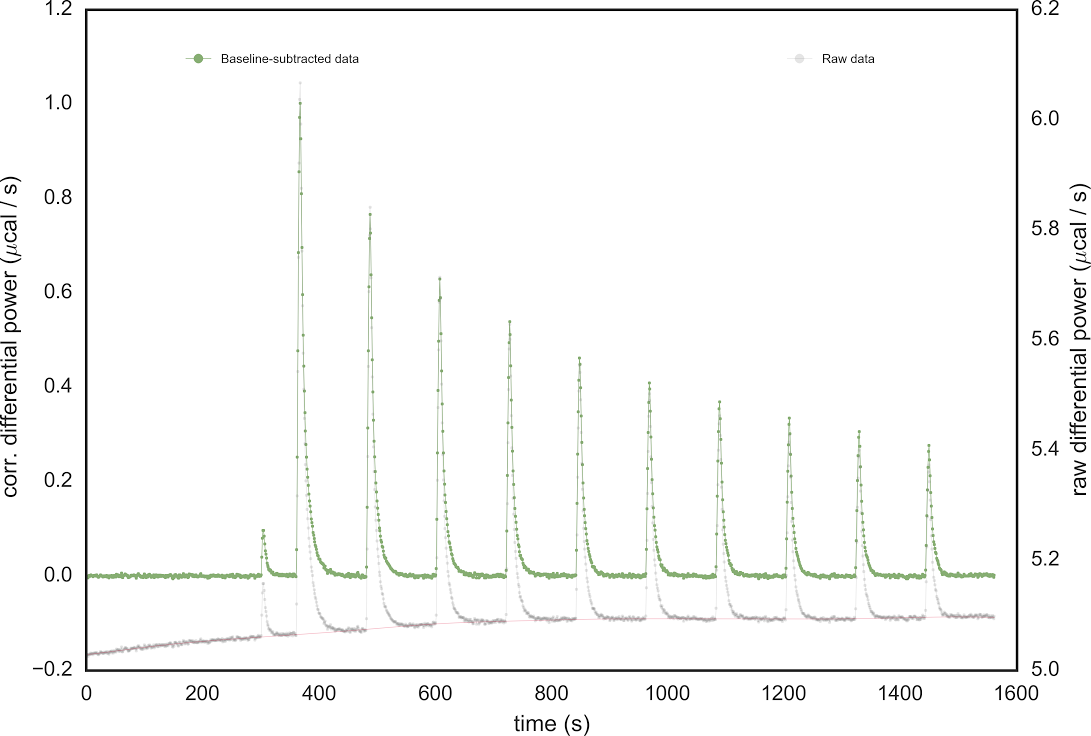
\includegraphics[width=\linewidth]{figures/itcexp.png}
\end{tikzfigure}
}

\block{Bayesian ITC}{
The posterior distribution is defined as
\begin{align}
	\mathcal{P}\left(\theta | \mathcal{D} \right) \propto  \mathcal{P}(\mathcal{D} | \theta) \mathcal{P}\left(\theta\right)
\end{align}
Here, $\mathcal{P}\left(\theta\right)$ is a prior density of our parameters:
\begin{align}
	\theta   =  \left\{ \Delta G_\mathrm{bind}, \Delta H_\mathrm{bind}, \Delta H_0, [\mathrm{X_{syr}}], [\mathrm{M_{cell}}], \sigma \right\} \quad,
\end{align}
which we use to propagate instrumental errors.
}



\block{Reliable baseline estimates}{
\begin{tikzfigure}[We apply Gaussian process regression to increase the reliability of our baseline estimates, using scikit learn~\autocite{Pedregosa2011a}.]
 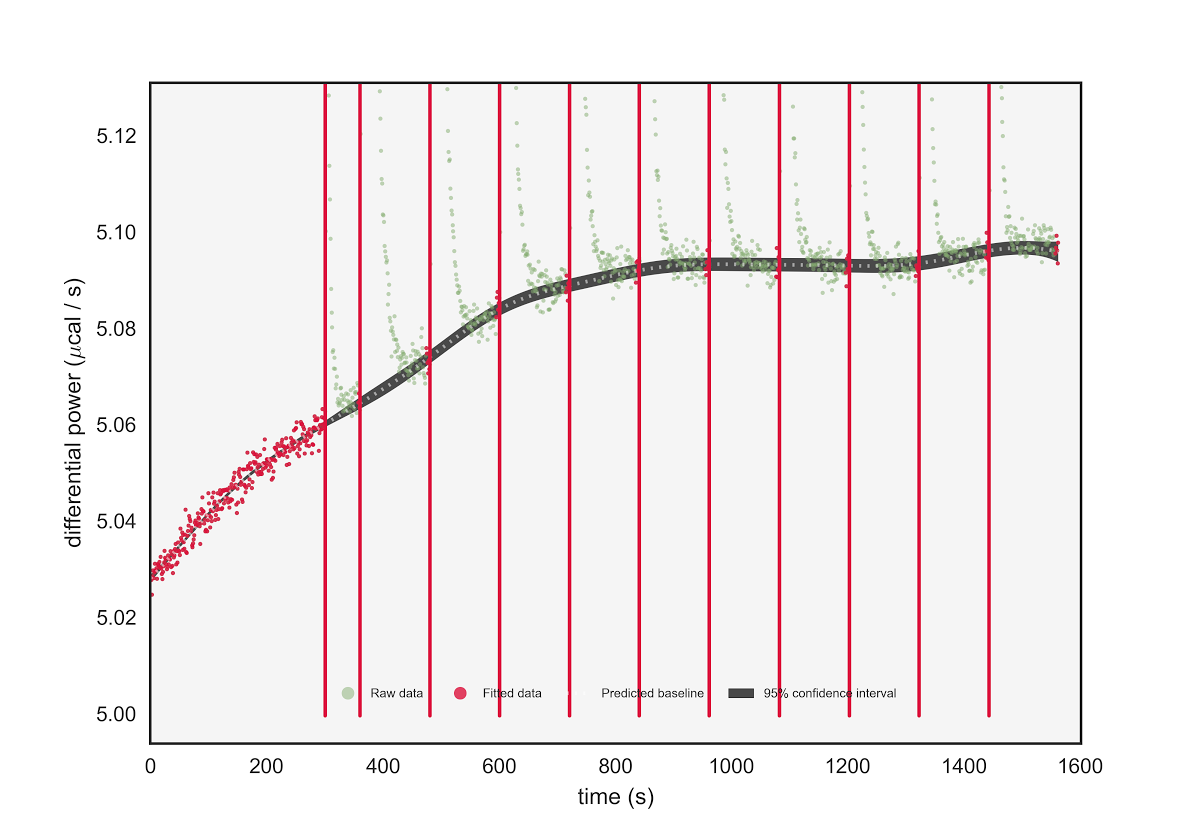
\includegraphics[width=\linewidth]{figures/baseline.png}
\end{tikzfigure}
}



 % SECOND column
\column{0.33}


\block{Uncertainty estimation}{
	\begin{tikzfigure}[ \small Binding measurements of CBS to bovine carbonic anhydrase II from the ABRF-MIRG'2 study.  A: Stoichiometry. B: Association constant. C: Binding enthalpy. D: Extinction coefficient of CBS, as reported by 14 participants~\autocite{Myszka2003a}.]
	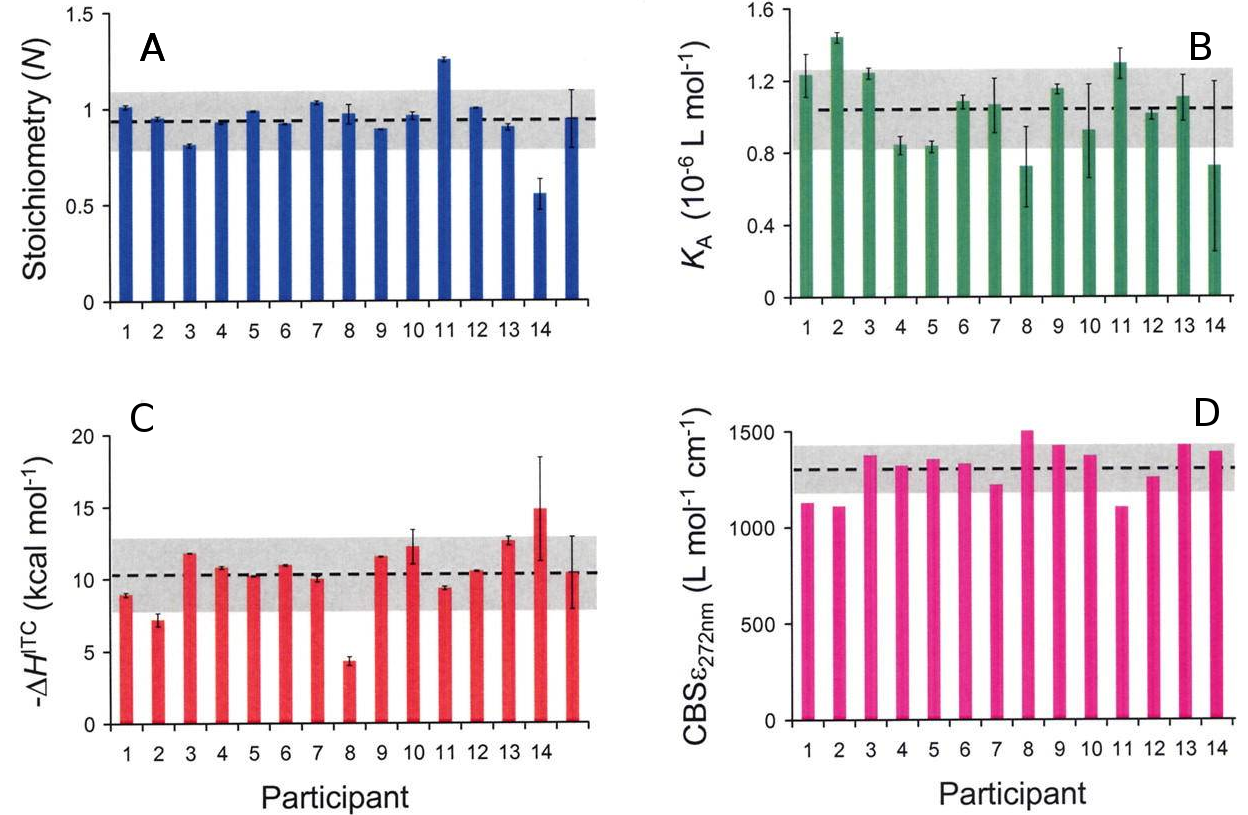
\includegraphics[width=\linewidth]{figures/cbs_ca_II.PNG}
	\end{tikzfigure}

}


\block[]{MCMC sampling}{
  \begin{tikzfigure}[An example distribution sampled for the syringe concentration using pymc~\autocite{Patil2010a}.]
   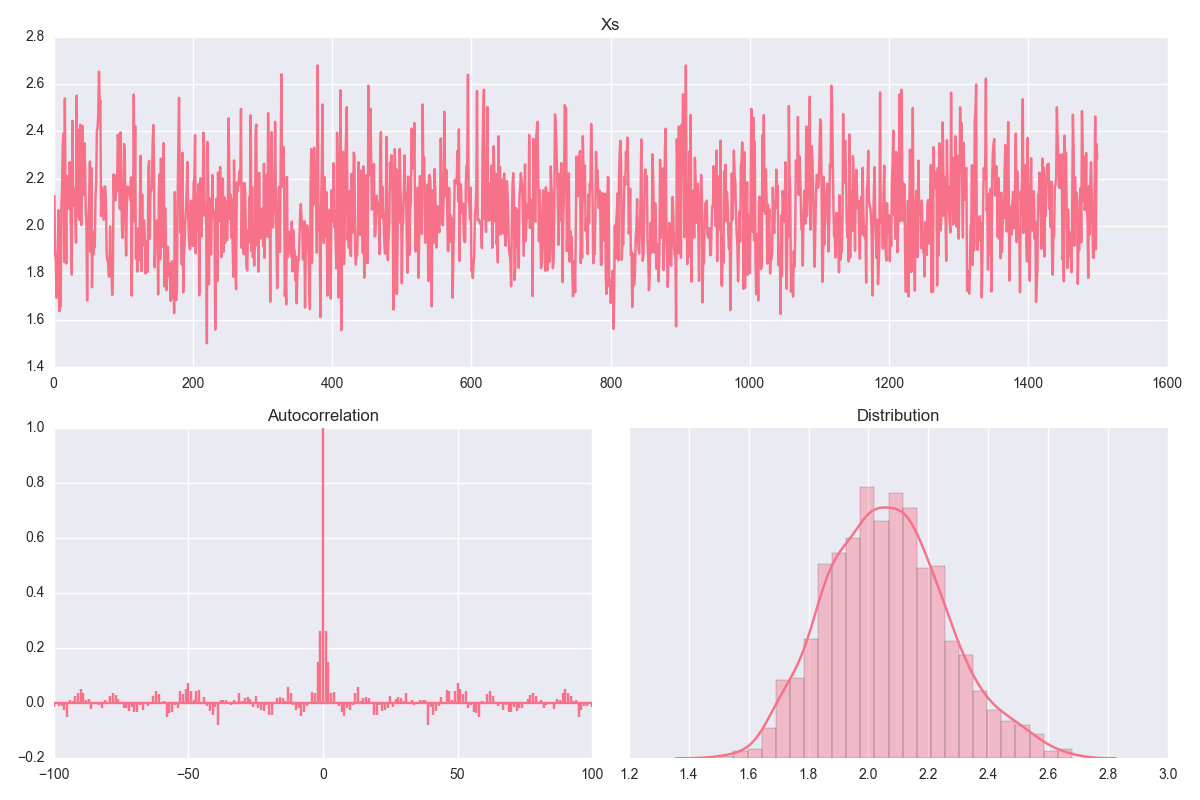
\includegraphics[width=\linewidth]{figures/sampling.png}
  \end{tikzfigure}

}


\block[]{Conclusions}{\normalsize
\begin{itemize}
	\item Not propagating errors in concentrations leads to large underestimation of uncertainty.
	\item Using Bayesian inference, we can incorporate prior information into our modeling
	\item MCMC will then give us posterior distributions with more accurate uncertainty estimates
	\item This allows us to use ITC experiments as a means of validating free energy calculations
\end{itemize}
}


% Third column
\column{0.33}



\block{Observation model}{
\vspace{0.5in}
We model the integrated heats as being samples from a normal distribution $\mathcal{N}$,
\begin{align}
q_n^\mathrm{obs} \sim \mathcal{N}(q_n^\mathrm{true}, \sigma^2) \quad ,
\end{align}
with the true heats $q_n^\mathrm{true}$ as a mean, with a variance of $\sigma^2$.
\vspace{0.9in}
}



\block{Posterior predictions}{
\begin{tikzfigure}[\small Our observations (red dots) and our sampled posterior heats (violins) provide us with new estimates plus credible intervals. Model traces are shown as dotted lines.]
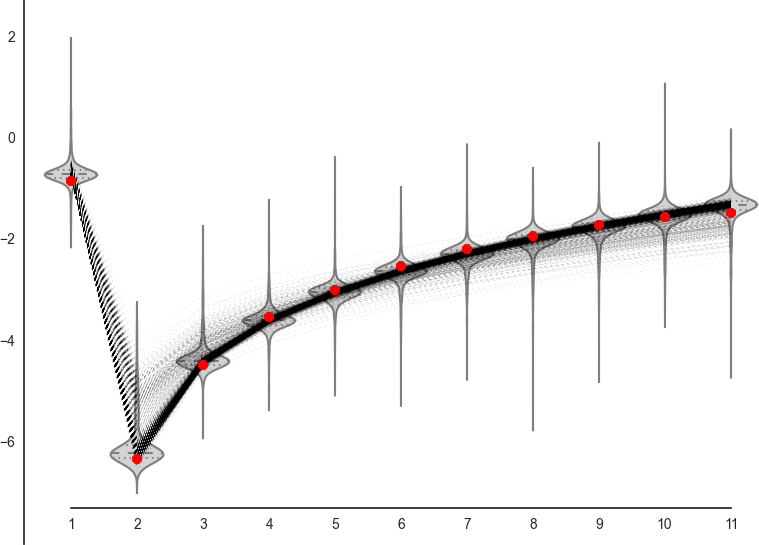
\includegraphics[width=\linewidth]{figures/postpredictive.png}
\end{tikzfigure}
\vspace{0.5in}
}

\block[]{References}{\printbibliography[heading=none]
}



\end{columns}


\end{document}
